
%%% Template originaly created by Karol Kozioł (mail@karol-koziol.net) and modified for ShareLaTeX use

\documentclass[a4paper,11pt]{article}

\usepackage{amsmath}
\usepackage[T1]{fontenc}
\usepackage[utf8]{inputenc}
\usepackage{graphicx}
\usepackage[usenames,dvipsnames]{xcolor}

\usepackage{sansmath}
\renewcommand\familydefault{\sfdefault}
\usepackage{tgheros}

\usepackage{amsmath,amssymb,amsthm,textcomp}
\usepackage{enumerate}
\usepackage{multicol}
\usepackage{tikz}
\usetikzlibrary{shapes, positioning}

\usepackage{geometry}
\geometry{total={210mm,297mm},
left=25mm,right=25mm,%
bindingoffset=0mm, top=20mm,bottom=20mm}


\linespread{1.3}

\newcommand{\linia}{\rule{\linewidth}{0.5pt}}

% custom theorems if needed
\newtheoremstyle{mytheor}
    {1ex}{1ex}{\normalfont}{0pt}{\scshape}{.}{1ex}
    {{\thmname{#1 }}{\thmnumber{#2}}{\thmnote{ (#3)}}}

\theoremstyle{mytheor}
\newtheorem{defi}{Definition}

% my own titles
\makeatletter
\renewcommand{\maketitle}{
\begin{center}
\vspace{2ex}
{\huge \textsc{\@title}}
\vspace{1ex}
\\
\linia\\
\@author \hfill \@date
\vspace{4ex}
\end{center}
}
\makeatother
%%%

% custom footers and headers
\usepackage{fancyhdr}
\pagestyle{fancy}
\lhead{}
\chead{}
\rhead{}
\lfoot{Automatic~Verification Assignment \#3}
\cfoot{}
\rfoot{Page \thepage}
\renewcommand{\headrulewidth}{0pt}
\renewcommand{\footrulewidth}{0pt}
%

% all section titles centered and bolded
\usepackage{sectsty}
\allsectionsfont{\bfseries\large}
%
% add section label
\renewcommand\thesection{Problem~\arabic{section}:}
\renewcommand\thesubsection{(\alph{subsection})}
%

%%%----------%%%----------%%%----------%%%----------%%%

\begin{document}

\title{Homework Assignment~\#3}

\author{R02943142 Hsieh, Chiao}

\maketitle

\section{Binary Decision Diagram}
Below is a binary decision diagram (BDD) where a true branch is represented by a solid line and a false branch by a dotted line.

\begin{center}
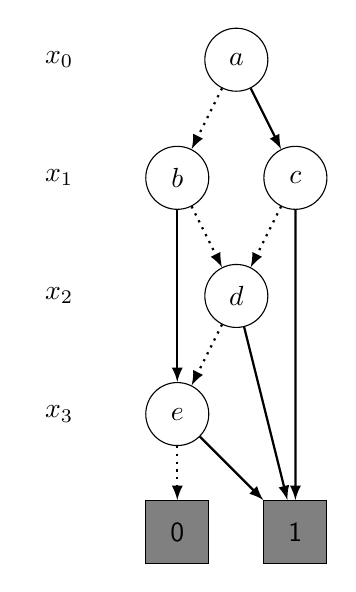
\begin{tikzpicture}[
  scale=1.5,
  every node/.style = {draw, circle, minimum width=8mm, minimum height=8mm},
  const/.style = {rectangle, fill=Gray},
  edge_1/.style = {draw, ->, >=latex, thick},
  edge_0/.style = {edge_1, dotted},
]
  \node[const] (0) at (0,0) {0};
  \node[const] (1) at (1,0) {1};

  \node[draw=none] (x0) at (-1,4) {$x_0$};
  \node[draw=none] (x1) at (-1,3) {$x_1$};
  \node[draw=none] (x2) at (-1,2) {$x_2$};
  \node[draw=none] (x3) at (-1,1) {$x_3$};

  \node (a) at (0.5, 4) {$a$};
  \node (b) at (0  , 3) {$b$};
  \node (c) at (1  , 3) {$c$};
  \node (d) at (0.5, 2) {$d$};
  \node (e) at (0  , 1) {$e$};

  \path [edge_0]
    (a) edge (b)
    (b) edge (d)
    (c) edge (d)
    (d) edge (e)
    (e) edge (0)
  ;
  \path [edge_1]
    (a) edge (c)
    (b) edge (e)
    (c) edge (1)
    (d) edge (1)
    (e) edge (1)
  ;

\end{tikzpicture}
\end{center}

\subsection{Recover \textit{in a systematic way} the boolean function represented by the BDD; use $x_0$, $x_1$, etc. to name the boolean variables.}

Answer.
\smallskip \\
We can compute the boolean function of a BDD node by recursively computing the functions of its co-factors and then deriving the function by the definition of  Shannon expansion.
Hence, we can derive the function of this BDD via computing the function of $a$. To simplify the procedure, the computation below demonstrates the bottom-up processing instead of top-down processing. 

\begin{equation*}
  \begin{array}{rl}
    f(e) &= \bar{x_3} \cdot f(0) + x_3 \cdot f(1) \\
         &= x_3 \\
    f(d) &= \bar{x_2} \cdot f(e) + x_2 \cdot f(1) \\
         &= \bar{x_2} \cdot x_3 + x_2 \\
    f(c) &= \bar{x_1} \cdot f(d) + x_1 \cdot f(1) \\
         &= \bar{x_1} \cdot (\bar{x_2} \cdot x_3 + x_2) + x_1 \\
    f(b) &= \bar{x_1} \cdot f(d) + x_1 \cdot f(e) \\
         &= \bar{x_1} \cdot (\bar{x_2} \cdot x_3 + x_2) + x_1 \cdot x_3\\
    f(a) &= \bar{x_0} \cdot f(b) + x_0 \cdot f(c) \\
         &= \bar{x_0} \cdot (\bar{x_1} \cdot (\bar{x_2} \cdot x_3 + x_2) + x_1 \cdot x_3) + x_0 \cdot (\bar{x_1} \cdot (\bar{x_2} \cdot x_3 + x_2) + x_1)
  \end{array}
\end{equation*}

\subsection{Draw a BDD (in canonical form) for the same function but with a different variable ordering: 1, 2, 3, 0.}
Answer.
\smallskip \\
The BDD for the same function but with ordering, (1, 2, 3, 0), is shown below.

\begin{center}
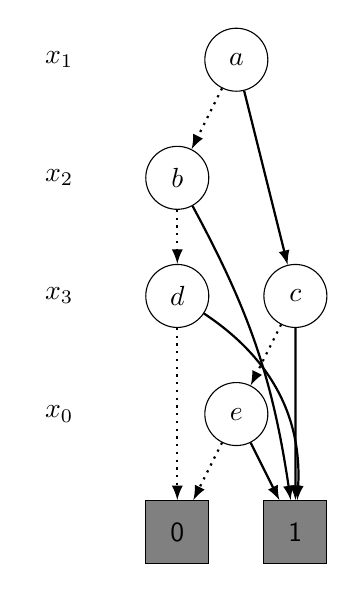
\begin{tikzpicture}[
  scale=1.5,
  every node/.style = {draw, circle, minimum width=8mm, minimum height=8mm},
  const/.style = {rectangle, fill=Gray},
  edge_1/.style = {draw, ->, >=latex, thick},
  edge_0/.style = {edge_1, dotted},
]
  \node[const] (0) at (0,0) {0};
  \node[const] (1) at (1,0) {1};

  \node[draw=none] (x1) at (-1,4) {$x_1$};
  \node[draw=none] (x2) at (-1,3) {$x_2$};
  \node[draw=none] (x3) at (-1,2) {$x_3$};
  \node[draw=none] (x0) at (-1,1) {$x_0$};
  
  \node (a) at (0.5, 4) {$a$};
  \node (b) at (  0, 3) {$b$};
  \node (c) at (  1, 2) {$c$};
  \node (d) at (  0, 2) {$d$};
  \node (e) at (0.5, 1) {$e$};

  \path [edge_0]
    (a) edge (b)
    (b) edge (d)
    (c) edge (e)
    (d) edge (0)
    (e) edge (0)
  ;
  \path [edge_1]
    (a) edge (c)
    (b) edge [bend left=10] (1)
    (c) edge (1)
    (d) edge [bend left] (1)
    (e) edge (1)
  ;

\end{tikzpicture}
\end{center}

\section{Fixpoint of CTL formula}
Consider symbolic model checking of CTL on finite Kripke structures. Prove that, for any CTL formula $f$, the following statements hold:

\subsection{The set of states satisfying AF$f$ is the least fixpoint of the function \\
$\tau(\mathit{Z}) = f \vee \textbf{AX}\mathit{Z}$.}
Answer.
\smallskip \\
To prove the statement, we first prove $\tau(Z) = f \vee \textbf{AX}Z$ is monotonic.
That is, if $P_1 \subseteq P_2$, we have to show that $\tau(P_1) \subseteq \tau(P_2)$. 

\noindent Proof:

Consider any state $s \in \tau(P_1)$, either $s \models f$ or all successors of $s$ are in $P_1$. If $s \models f$, then $s \in f \vee \textbf{AX}Z = \tau(P_2)$. If all successors of $s$ are in $P_1$, then all these successors are also in $P_2$ since $P_1 \subseteq P_2$. Hence, $s \in \tau(P_2)$ as well, and we proved that $\tau(P_1) \subseteq \tau(P_2)$.

\bigskip
\noindent
Second, we need to prove that $\textbf{AF}f$ is a fixpoint of $\tau(Z)$.
In other words, $\textbf{AF}f = \tau(\textbf{AF}f)$.

\noindent Proof:

Let $s_0 \models \textbf{AF}f$.
By definition, for each path $s_0, s_1, \dots$ in $M$, there is a state $s_k$
in each path such that $s_k \models f$. If $k=0$, then $s_0 \models f \subseteq
f \vee \textbf{AX\ AF}f$. If $k>=1$, then $s_1 \models \textbf{AF}f$ for all
paths starting from $s_0$. This implies that $s_0 \models \textbf{AX\ AF}f
\subseteq f \vee \textbf{AX\ AF}f$. Hence, we proved $\textbf{AF}f \subseteq
\tau(\textbf{AF}f)$.

In the other direction, we assume $s_0 \models f \vee \textbf{AX\ AF}f$. 
If $s_0 \models f$, then $s_0 \models \textbf{AF}f$. Otherwise, when $s_0
\models \textbf{AX\ AF}f$, this implies $s_1 \models \textbf{AF}f$ for any
successor $s_1$ of $s_0$. This means there is a state $s_k \models f$ in
any path starting from $s_1$ and therefore any path from $s_0$. That is, 
$s_0 \models \textbf{AF}f$, and we proved $\tau(\textbf{AF}f) \subseteq
\textbf{AF}f$.

Since $\textbf{AF}f \subseteq \tau(\textbf{AF}f)$ and $\tau(\textbf{AF}f) 
\subseteq \textbf{AF}f$. We know $\textbf{AF}f = \tau(\textbf{AF}f)$.

\bigskip
\noindent
Finally, as $\tau(Z)$ is monotonic, we know $\tau(Z)$ is also 
$\bigcup$-continuous. Thus, we can explain why $\textbf{AF}f$ is the least
fixpoint by simply proving $\bigcup_{i}\tau^{i}(\bot) = \textbf{AF}f$.

\noindent Proof:

We first prove $\bigcup_{i}\tau^{i}(\bot) \subseteq \textbf{AF}f$, and it is
sufficient to show that $\forall i, \tau^{i}(\bot) \subseteq \textbf{AF}f$.
The proof is achieved by induction on $i$.

\noindent Base case: $\tau^{0}(\bot) = \bot \subseteq \textbf{AF}f$

\noindent Inductive Step:

Assuming $\tau^{k}(\bot) \subseteq \textbf{AF}f$ for any $k$, we know 
$\tau^{k+1}(\bot) \subseteq \tau(\textbf{AF}f)$ due to the monotonicity.
Besides, $\because \tau(\textbf{AF}f) = \textbf{AF}f \therefore 
\tau^{k+1}(\bot) \subseteq \textbf{AF}f$.

\noindent By induction, we proved $\forall i, \tau^{i}(\bot) \subseteq \textbf{AF}f$,
and therefore $\bigcup_{i}\tau^{i}(\bot) \subseteq \textbf{AF}f$.

\medskip
\noindent Then, we prove $\textbf{AF}f \subseteq \bigcup_{i}\tau^{i}(\bot)$

If state $s_1 \models \textbf{AF}f$, for each path $s_1, s_2, \dots$ in $M$, 
there is a state $s_j$ in each path such that $s_j \models f$. We claim that
$s_1 \in \tau^{j}(\bot)$ always holds.

\noindent Base case: For $j=1, s_1=s_j \implies s_1 \models f \subseteq f \vee
\textbf{AX\ AF} \bot. \therefore s_1 \in \tau^{j}(\bot)$

\noindent Inductive Step:

For $j+1>1$, since $s_1 \models \textbf{AF}f$ and $s_1 \not\models f$, any
successor $s_2$ of $s_1$ must also satisfy that $s_2 \models \textbf{AF}f$.
From induction hypothesis, we know $\forall s_2, (s_1, s_2) \in R, 
s_2 \in \tau^{j}(\bot)$. \\
$\therefore s_1 \models \textbf{AX}(\tau^{j-1}(\bot)) \subseteq 
f \vee \textbf{AX}(\tau^{j}(\bot)) = \tau^{j+1}(\bot)$. That is, 
$s_1 \in \tau^{j+1}(\bot)$, and hence by induction $s_1 \in \tau^{j}(\bot)$ 
if $s_j \models f$ in that path.

Further, we conclude that $s_1 \in \bigcup_{i}\tau^{i}(\bot)$ since all possible
$j$ are included for all paths starting from $s_1$, so $\textbf{AF}f \subseteq
\bigcup_{i}\tau^{i}(\bot)$.

\medskip \noindent
$\because \bigcup_{i}\tau^{i}(\bot) \subseteq \textbf{AF}f$ and 
$\textbf{AF}f \subseteq \bigcup_{i}\tau^{i}(\bot)$
$\therefore \textbf{AF}f = \bigcup_{i}\tau^{i}(\bot)$ which means
$\textbf{AF}f$ is the lfp of $\tau(Z)$.

\subsection{The set of states satisfying AG$f$ is the greatest fixpoint of the 
function \\ 
$\tau(\mathit{Z}) = f \wedge \textbf{AX}\mathit{Z}$}
Answer.
\smallskip \\
In this problem, we show the equivalence by translating the formulae into 
$\mu$-calculus. First, we rewrite the CTL formulae with only \textbf{EX, EU, EG}
operators.
\begin{equation*}
  \begin{array}{ll}
    f \wedge \textbf{AX}Z &= f \wedge \neg\textbf{EX} \neg Z \\
    \textbf{AG}f &= \neg \textbf{EF} \neg f = \neg \textbf{E}[ true \textbf{U} \neg f ]
  \end{array}
\end{equation*}

\noindent Then, we translate these two formulae via $\mathtt{Tr}(f)$ algorithm.
\begin{equation*}
  \begin{array}{ll}
    \nu Z. f \wedge \textbf{AX}Z 
       &= \nu Z.f \wedge \neg\textbf{EX} \neg Z 
        = \nu Z.f \wedge \neg(\langle a\rangle \neg Z)
        = \nu Z.f \wedge ([a] Z)\\
    \mathtt{Tr}(\textbf{AG}f)
       &= \mathtt{Tr}(\neg \textbf{E}[ true \textbf{U} \neg f ])
        = \neg \mathtt{Tr}(\textbf{E}[ true \textbf{U} \neg f ]) \\
       &= \neg \mu Z.(\mathtt{Tr}(\neg f) \vee (\mathtt{Tr}(true) \wedge \langle a\rangle Z) )
        = \neg \mu Z.(\neg f \vee \langle a\rangle Z)\\
       &= \nu Z.\neg(\neg f \vee \langle a\rangle \neg Z)
        = \nu Z.(f \wedge \neg \langle a\rangle \neg Z)
        = \nu Z.f \wedge ([a] Z)\\
  \end{array}
\end{equation*}
Hence, we proved that $\textbf{AG}f$ is the greatest fixpoint of $\tau(Z)$.


\section{Symbolic Model Checking}
Consider a system with two processes (0 and 1) that repeatedly attempt to 
enter the critical section via the arbitration of a binary semaphore. This 
system may be modelled as the following Kripke structure. Use the symbolic 
CTL model checking algorithm in [CGP; Chapter 6] to compute the states that 
satisfy the CTL formula $\textbf{AG}((s_0 = e) \rightarrow \textbf{AF}(s_0 = c))$.
\medskip \\
Answer.
\smallskip \\
First, we define the encoding of states, $\phi: 2^3 \mapsto \{n_0\dotsc n_7\}$. We follow the
binary encoding of three boolean variables $\vec{x}=(x_2,x_1,x_0)$, i.e.,
$(0,0,0)\mapsto n_0, (0,0,1)\mapsto n_1, \dots, (1,1,1)\mapsto n_7$.
Following this encoding, the boolean representation of the transition relation,
$\hat{R}(\vec{x}, \vec{x'})$, is easily derived.
\begin{equation*}
\begin{array}{lclcl}
   \hat{R}(\vec{x}, \vec{x'})
      &=& \bar{x_2}\bar{x_1}\bar{x_0}(\bar{x_2'}\bar{x_1'}x_0' + \bar{x_2'}x_1'\bar{x_0'}) & \cdots & n_0 \mapsto \{n_1,n_2\}\\
      &+& \bar{x_2}\bar{x_1}x_0(\bar{x_2'}x_1'x_0' + x_2'\bar{x_1'}\bar{x_0'})             & \cdots & n_1 \mapsto \{n_3,n_4\}\\
      &+& \bar{x_2}x_1\bar{x_0}(x_2'\bar{x_1'}\bar{x_0'} + x_2'\bar{x_1'}x_0')             & \cdots & n_2 \mapsto \{n_4,n_5\}\\
      &+& \bar{x_2}x_1x_0(\bar{x_2'}\bar{x_1'}\bar{x_0'} + x_2'x_1'\bar{x_0'})             & \cdots & n_3 \mapsto \{n_0,n_6\}\\
      &+& x_2\bar{x_1}\bar{x_0}(x_2'x_1'\bar{x_0'} + x_2'x_1'x_0')                         & \cdots & n_4 \mapsto \{n_6,n_7\}\\
      &+& x_2\bar{x_1}x_0(\bar{x_2'}\bar{x_1'}\bar{x_0'} + x_2'x_1'x_0')                   & \cdots & n_5 \mapsto \{n_0,n_7\}\\
      &+& x_2x_1\bar{x_0}(\bar{x_2'}x_1'\bar{x_0'} + x_2'x_1'\bar{x_0'})                   & \cdots & n_6 \mapsto \{n_2,n_6\}\\
      &+& x_2x_1x_0(\bar{x_2'}\bar{x_1'}x_0' + x_2'x_1'x_0')                               & \cdots & n_7 \mapsto \{n_1,n_7\}\\
\end{array}
\end{equation*}
Also the boolean representation for each atomic proposition is listed below.
\begin{equation*}
  \begin{array}{llcl}
   L_{\mathtt{sem=1}} &= \bar{x_2}\bar{x_1}\bar{x_0} + \bar{x_2}\bar{x_1}x_0 
                       + \bar{x_2}x_1\bar{x_0} + x_2\bar{x_1}\bar{x_0}       & \cdots & (\mathtt{sem=1}) \mapsto \{n_0,n_1,n_2,n_4\}\\
   L_{\mathtt{sem=0}} &= \neg L_{\mathtt{sem}=1} \\
   L_{\mathtt{s_0=i}} &= \bar{x_2}\bar{x_1}\bar{x_0} + \bar{x_2}x_1\bar{x_0}
                       + x_2\bar{x_1}x_0                                     & \cdots & (\mathtt{s_0=i}) \mapsto \{n_0,n_2,n_5\}\\
   L_{\mathtt{s_0=e}} &= \bar{x_2}\bar{x_1}x_0 + x_2\bar{x_1}\bar{x_0}
                       + x_2x_1x_0                                           & \cdots & (\mathtt{s_0=e}) \mapsto \{n_1,n_4,n_7\}\\
   L_{\mathtt{s_0=c}} &= \bar{x_2}x_1x_0 + x_2x_1\bar{x_0}                   & \cdots & (\mathtt{s_0=c}) \mapsto \{n_3,n_6\}\\
   L_{\mathtt{s_1=i}} &= \bar{x_2}\bar{x_1}\bar{x_0} + \bar{x_2}\bar{x_1}x_0
                       + \bar{x_2}x_1x_0                                     & \cdots & (\mathtt{s_1=i}) \mapsto \{n_0,n_1,n_3\}\\
   L_{\mathtt{s_1=e}} &= \bar{x_2}x_1\bar{x_0} + x_2\bar{x_1}\bar{x_0}
                       + x_2x_1\bar{x_0}                                     & \cdots & (\mathtt{s_1=e}) \mapsto \{n_2,n_4,n_6\}\\
   L_{\mathtt{s_1=c}} &= x_2\bar{x_1}x_0 + x_2x_1x_0                         & \cdots & (\mathtt{s_1=c}) \mapsto \{n_5,n_7\}\\
  \end{array}
\end{equation*}
Then, we normalize the CTL formula.
\begin{equation*}
\begin{array}{ll}
   \textbf{AG}((s_0 = e) \rightarrow \textbf{AF}(s_0 = c))
      &= \neg \textbf{EF} \neg((s_0 = e) \rightarrow \neg \textbf{EG} \neg(s_0 = c)) \\
      &= \neg \textbf{EF} \neg( \neg(s_0 = e) \vee \neg \textbf{EG} \neg(s_0 = c)) \\
      &= \neg \textbf{EF} ((s_0 = e) \wedge \textbf{EG} \neg(s_0 = c)) \\
      &= \neg \textbf{E} [ \top \textbf{U} ((s_0 = e) \wedge \textbf{EG} \neg(s_0 = c))] \\
\end{array}
\end{equation*}
The algorithm in the textbook recursively calls \textit{Check} procedure to 
verify a property, but here we demonstrate the procedure in Bottom-up manner.
\begin{equation*}
 \begin{array}{l}
  \textit{Check}(\neg(s_0 = c)) = \neg L_{\mathtt{s_0=c}} \\
  \textit{Check}(\textbf{EG} \neg(s_0 = c)) = \textit{CheckEG}(\neg L_{\mathtt{s_0=c}})
 \end{array}
\end{equation*}
To compute $\textit{CheckEG}(\neg L_{\mathtt{s_0=c}})$, we derive the greatest
fixpoint of $\tau(Z) = \neg L_{\mathtt{s_0=c}} \wedge \textbf{EX} Z$.
\begin{equation*}
 \begin{array}{ll}
  \tau^{1}(\top) &= \neg L_{\mathtt{s_0=c}} \wedge \textbf{EX}(\top) = \neg L_{\mathtt{s_0=c}} \\
  \tau^{2}(\top) &= \neg L_{\mathtt{s_0=c}} \wedge \textbf{EX}(\neg L_{\mathtt{s_0=c}}) 
                  = \neg L_{\mathtt{s_0=c}} \wedge \top = \neg L_{\mathtt{s_0=c}} 
                  = \tau^{1}(\top) \\
 \end{array}
\end{equation*}
Hence, we find the greatest fixpoint, and 
$\textit{CheckEG}(\neg L_{\mathtt{s_0=c}}) = \neg L_{\mathtt{s_0=c}}$. Then,
\begin{equation*}
 \begin{array}{l}
  \textit{Check}((s_0 = e) \wedge \textbf{EG} \neg(s_0 = c)) 
     = L_{\mathtt{s_0 = e}} \cdot \neg L_{\mathtt{s_0=c}} = L_{\mathtt{s_0 = e}}\\
  \textit{Check}(\textbf{E}[\top \textbf{U}(s_0 = e) \wedge \textbf{EG} \neg(s_0 = c)])
     = \textit{CheckEU}(\top, L_{\mathtt{s_0 = e}})
 \end{array}
\end{equation*}
To derive $\textit{CheckEU}(\top, L_{\mathtt{s_0 = e}})$, we compute the least
fixpoint of $\tau(Z) = L_{\mathtt{s_0 = e}} \vee (\top \wedge\textbf{EX} Z)
= L_{\mathtt{s_0 = e}} \vee \textbf{EX} Z$.
\begin{equation*}
 \begin{array}{ll}
  \tau^{1}(\bot) &
     = L_{\mathtt{s_0 = e}} \vee \textbf{EX}(\bot) = L_{\mathtt{s_0 = e}} \\
  \tau^{2}(\bot) &
     = L_{\mathtt{s_0 = e}} \vee \textbf{EX}(L_{\mathtt{s_0 = e}})
     = L_{\mathtt{s_0 = e}} \vee L_{\mathtt{s_0 = e}} \vee L_{\mathtt{s_0 = i}}
     = L_{\mathtt{s_0 = e}} \vee L_{\mathtt{s_0 = i}} \\
  \tau^{3}(\bot) &
     = L_{\mathtt{s_0 = e}} \vee \textbf{EX}(L_{\mathtt{s_0 = e}} \vee L_{\mathtt{s_0 = i}})
     = L_{\mathtt{s_0 = e}} \vee \top = \top \\
 \end{array}
\end{equation*} 
The least fixpoint is found, and $\textit{CheckEU}(\top, L_{\mathtt{s_0 = e}}) = \top$. Continue
\begin{equation*}
 \begin{array}{l}
  \textit{Check}(\neg\textbf{E}[\top \textbf{U}(s_0 = e) \wedge \textbf{EG} \neg(s_0 = c)])\\
    = \neg \top \\
    = \bot \\
 \end{array}
\end{equation*}
Therefore, no state in the system satisfies the CTL property,
$\textbf{AG}((s_0 = e) \rightarrow \textbf{AF}(s_0 = c))$.
\end{document}